\section{Dataset Description and EDA}
\label{sec:dataset}

\subsection{Dataset}
We use Fashion-MNIST~\cite{xiao2017fashion}: 28$\times$28 grayscale images of clothing in 10 classes, with an official split of 60{,}000 training and 10{,}000 test images. Validation data are a stratified 10\% of the official training images (6{,}000 images, 600 per class, seed 42), leaving 54{,}000 images for training. The 10{,}000 official test images are read only for the integrity checks in the loading step (shapes, data types, pixel range and class counts), from which nothing is selected or tuned, and for the report-only duplicate check, which runs after the final evaluation. Every other statistic in this section uses the official training images: the class distribution uses all 60{,}000, and the pixel statistics, PCA and class-mean analyses use the 54{,}000-image training split. Loading checks confirmed uint8 images with pixel values from 0 to 255, int64 labels from 0 to 9, and class names aligned with torchvision. The official training set is exactly balanced, with 6{,}000 images per class (Fig.~\ref{fig:classdist}), and the test set has 1{,}000 per class.

\subsection{Data quality}
We hashed the raw bytes of every image and found no exact duplicates within the training set, within the test set, between training and test, or between our 54{,}000-image training split and the 6{,}000-image validation split. This check finds only byte-identical images; near-duplicates were not examined.

\subsection{Pixel statistics}
On the 54{,}000-image training split, the mean pixel value is 0.2862 and the standard deviation is 0.3532 (scale 0--1). Exactly 50.21\% of all pixels are zero, which reflects the black background. Mean intensity differs by class, from 0.137 for Sandal and 0.168 for Sneaker to 0.377 for Pullover and 0.385 for Coat. Fig.~\ref{fig:means} shows the mean image of each class.

\subsection{Structure of the classes}
\textbf{Class means.} The closest pairs of class mean images (Euclidean distance on pixels scaled to 0--1; all pairs are in Fig.~\ref{fig:centroid}) are Pullover--Coat (2.473), Pullover--Shirt (2.677), Coat--Shirt (2.990), T-shirt/top--Shirt (3.685) and Sandal--Sneaker (3.823). These distances are descriptive; we do not claim they predict classifier errors, and they are compared with the real confusion matrices later.

\textbf{PCA.} PCA fitted on the training split only gives 71.98\% of the variance in the first 10 components and 86.25\% in the first 50. The first two components explain 28.99\% and 17.77\% (46.76\% together). In the two-dimensional projection of 5{,}000 stratified training images (Fig.~\ref{fig:pca}), Shirt, Pullover and Coat overlap heavily, T-shirt/top overlaps with Shirt and Dress, Trouser forms a compact cluster, and Sandal and Sneaker overlap strongly. PCA is linear and unsupervised and the plot shows less than half of the variance, so overlap here does not show that the classes are inseparable.

\textbf{Visual inspection.} In a panel of eight random training images per class (Fig.~\ref{fig:panel}), Shirt images vary widely in pattern and sleeve length. By eye, some plain Shirt images resemble T-shirt/top and some plain long-sleeved Coat images resemble Pullover. This is an impression from 32 images, not a measured rate.

\subsection{Sanity baselines}
Two floor references on the validation set: always predicting the majority class gives accuracy 0.100 and macro-F1 0.0182, as expected for 600 of 6{,}000 validation images per class; nearest class mean gives accuracy 0.692 and macro-F1 0.6882. Both are floors and are not part of the nine-model comparison.

\subsection{Limits of 28$\times$28 grayscale}
Each image has only 784 grey values. We hypothesise that this removes fine detail such as buttons, collars and fabric texture, which may make the upper-body classes look alike, and that missing colour removes a further cue. We also hypothesise that images of this style may not match real inventory photos taken at varied size, angle and background. These statements were not tested in this phase.

\begin{figure}[t]
\centering
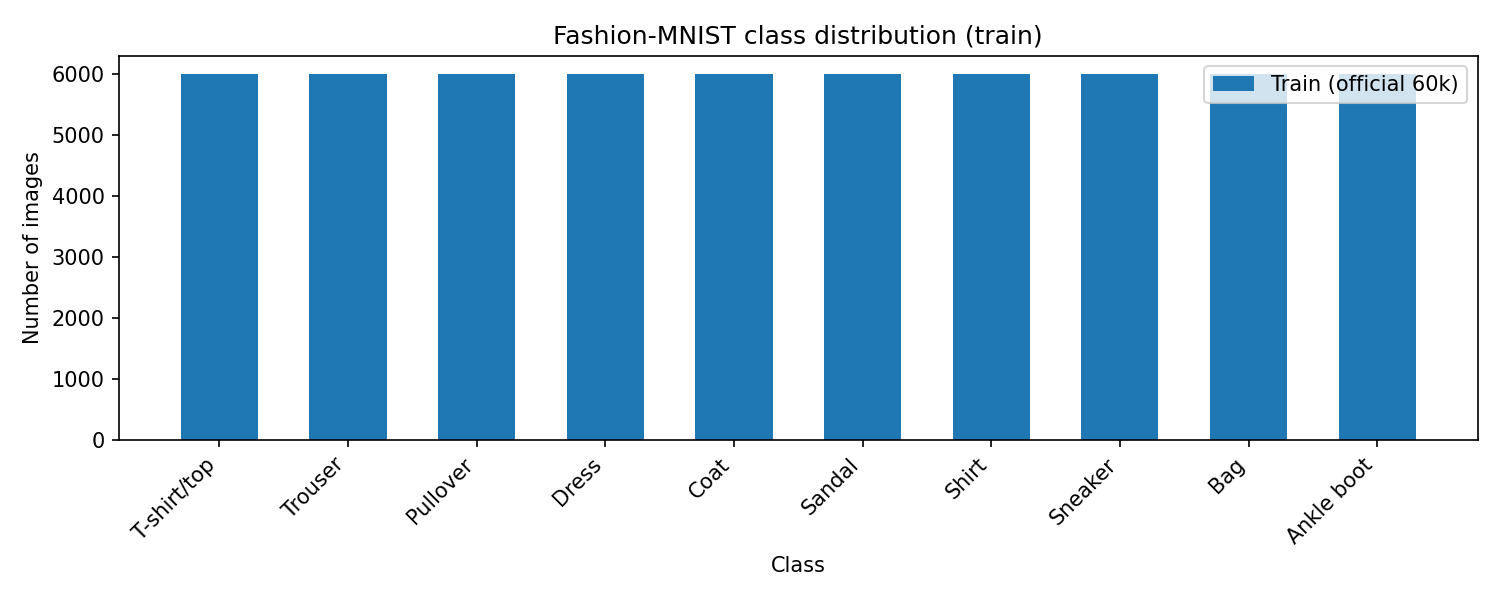
\includegraphics[width=\columnwidth]{figures/eda_class_distribution.png}
\caption{Number of images per class in the official training set (60{,}000 images).}
\label{fig:classdist}
\end{figure}

\begin{figure}[t]
\centering
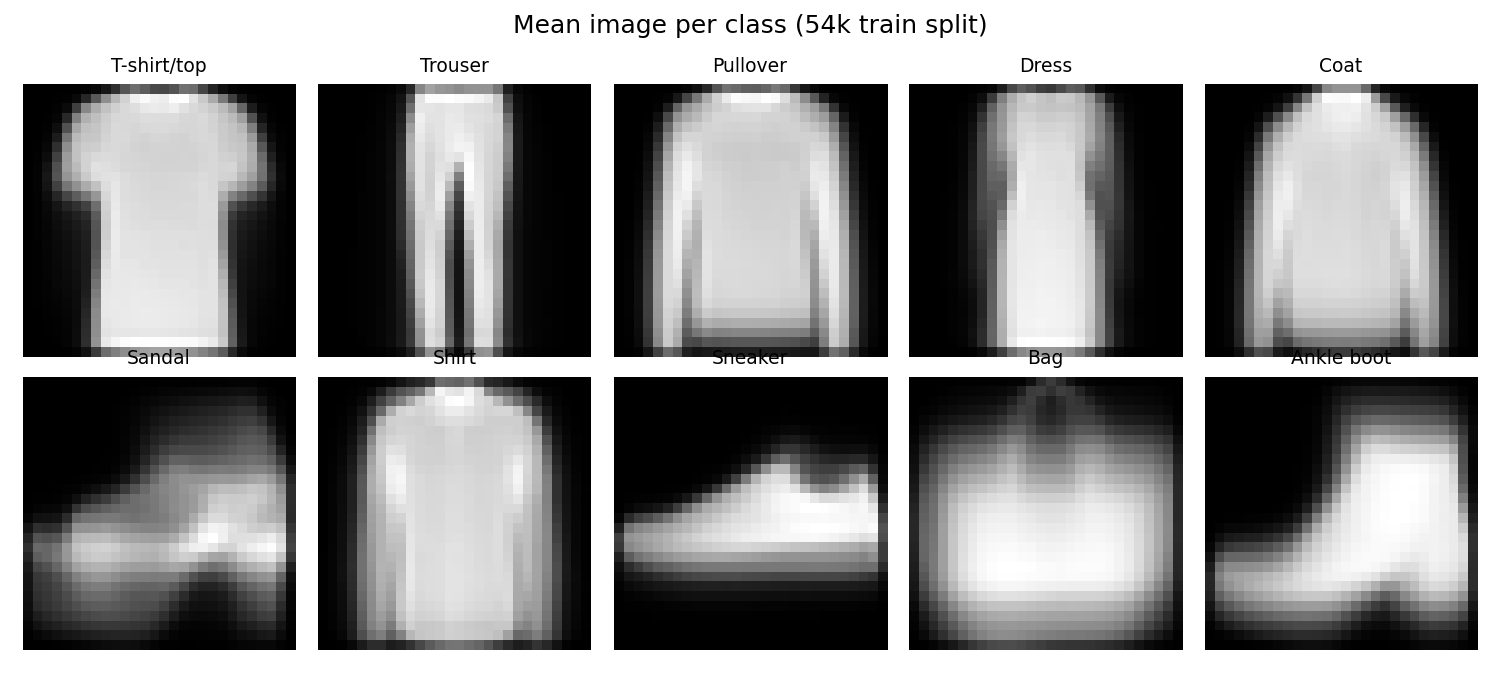
\includegraphics[width=\columnwidth]{figures/eda_mean_images.png}
\caption{Mean image of each class on the 54{,}000-image training split.}
\label{fig:means}
\end{figure}

\begin{figure}[t]
\centering
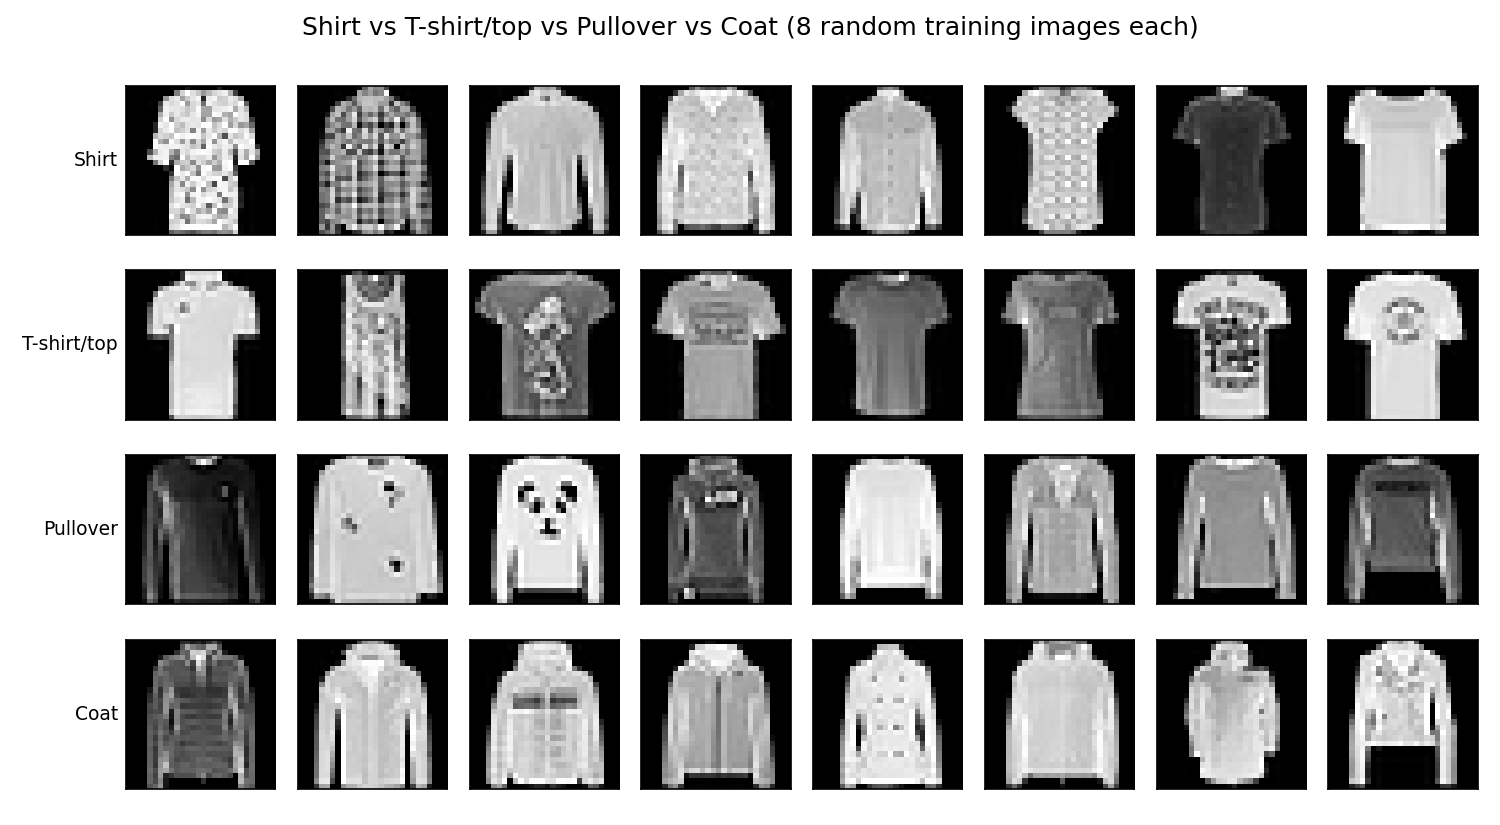
\includegraphics[width=\columnwidth]{figures/eda_confusable_panel.png}
\caption{Eight random training images each of Shirt, T-shirt/top, Pullover and Coat.}
\label{fig:panel}
\end{figure}

\begin{figure}[t]
\centering
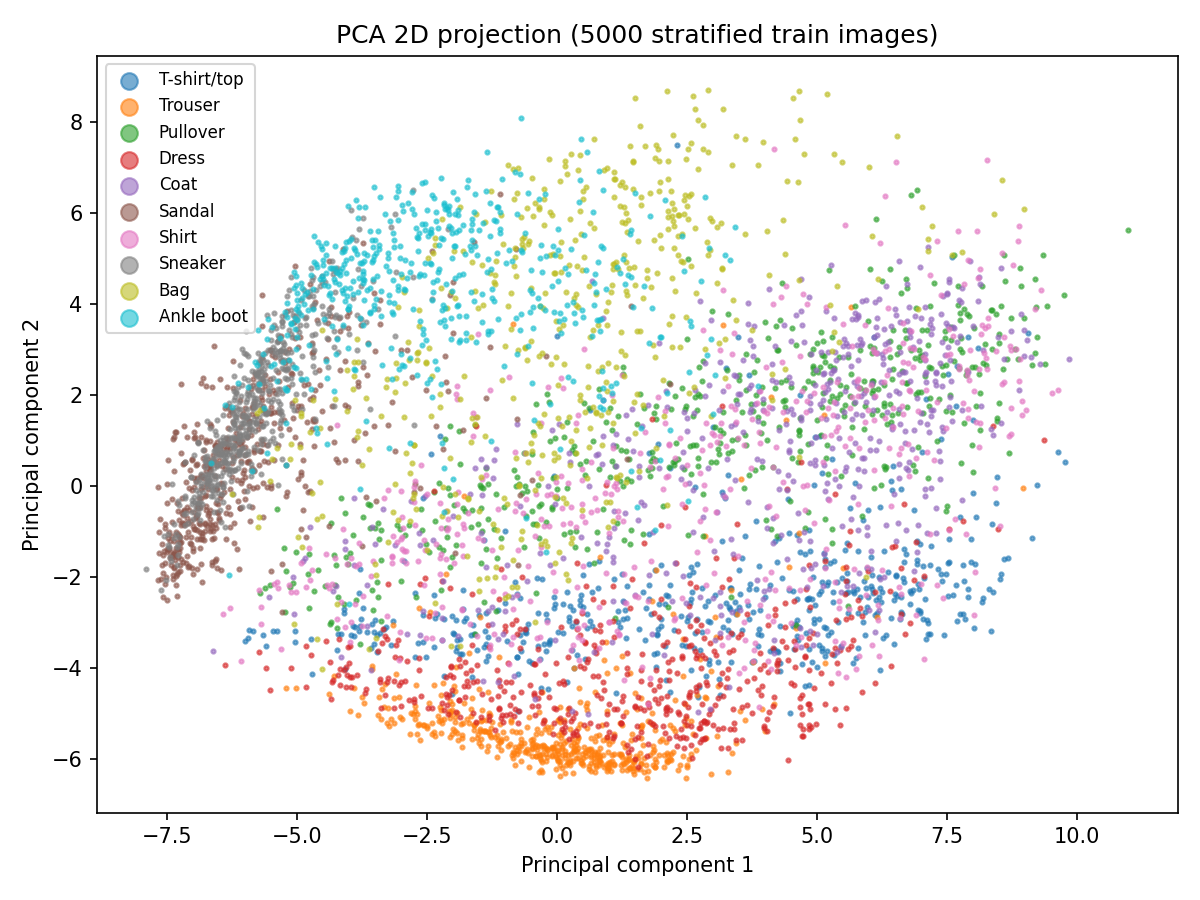
\includegraphics[width=\columnwidth]{figures/eda_pca_scatter.png}
\caption{PCA projection onto the first two components of 5{,}000 stratified training images, coloured by class. PCA was fitted on the training split only.}
\label{fig:pca}
\end{figure}

\begin{figure}[t]
\centering
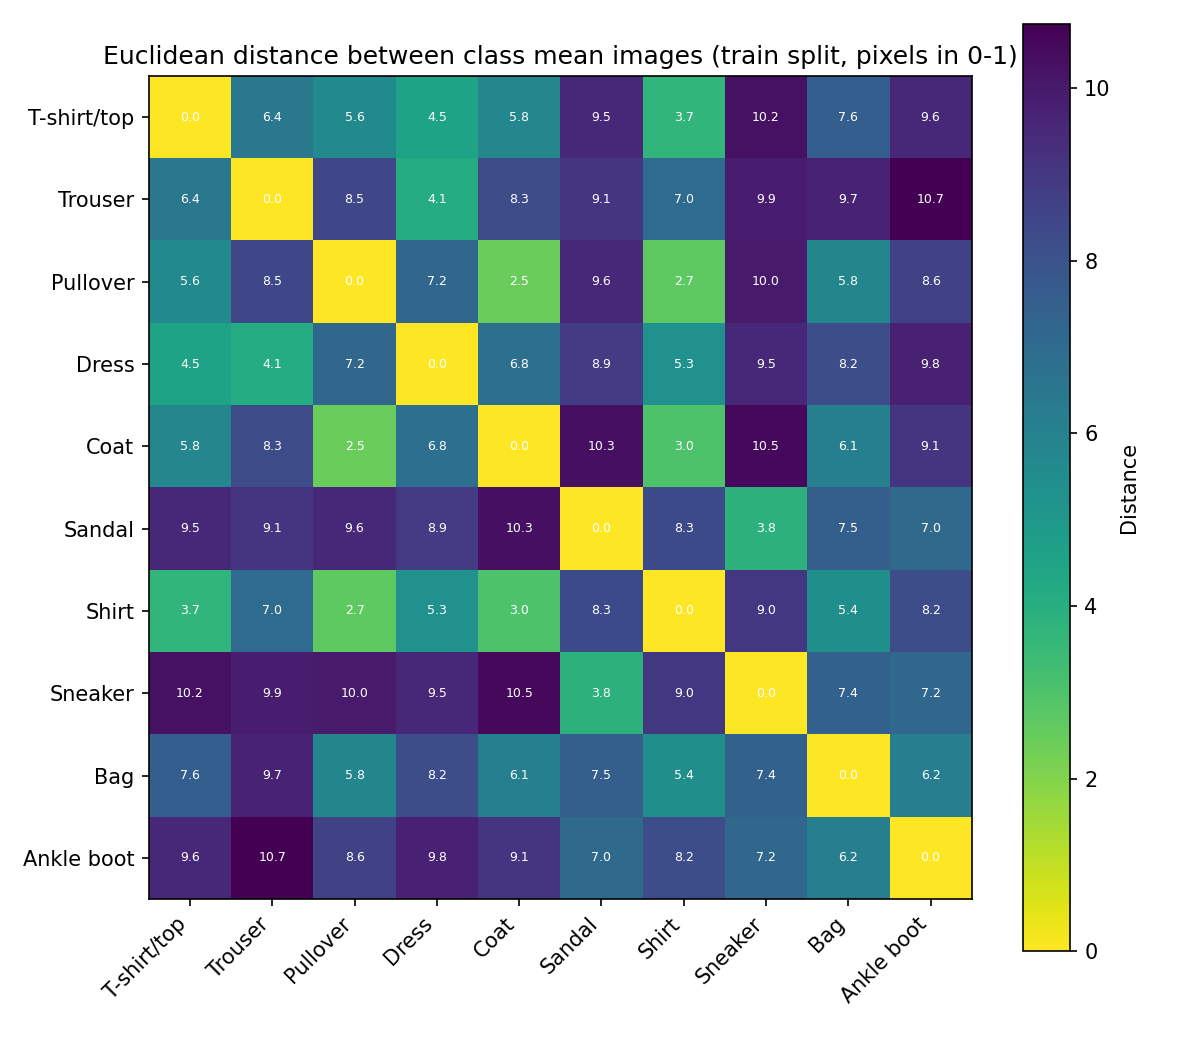
\includegraphics[width=\columnwidth]{figures/eda_centroid_heatmap.png}
\caption{Euclidean distance between class mean images on the training split (pixels scaled to 0--1).}
\label{fig:centroid}
\end{figure}
